\documentclass{article}

% packages for math
\usepackage{amsthm}
\usepackage{amsmath}
\usepackage{amssymb}
\usepackage{amsfonts}

% package for including images
\usepackage{graphicx}

% TAKEN FROM OVERLEAF DOCUMENTATION
% https://www.overleaf.com/learn/latex/Code_listing
\usepackage{listings}
\lstset{language=Python}
\usepackage{xcolor}
\definecolor{codegreen}{rgb}{0,0.6,0}
\definecolor{codegray}{rgb}{0.5,0.5,0.5}
\definecolor{codepurple}{rgb}{0.58,0,0.82}
\definecolor{backcolour}{rgb}{0.95,0.95,0.92}
\lstdefinestyle{mystyle}{
  backgroundcolor=\color{backcolour},
  commentstyle=\color{codegreen},
  keywordstyle=\color{magenta},
  numberstyle=\tiny\color{codegray},
  stringstyle=\color{codepurple},
  basicstyle=\ttfamily\footnotesize,
  breakatwhitespace=false,
  breaklines=true,
  captionpos=b,
  keepspaces=true,
  numbers=left,
  numbersep=5pt,
  showspaces=false,
  showstringspaces=false,
  showtabs=false,
  tabsize=2
}
\lstset{style=mystyle}

% environment for solutions
\theoremstyle{remark}
\newtheorem*{solution}{Solution}

% capital letters for problem parts
\renewcommand{\theenumi}{\Alph{enumi}}

% no page numbers
\pagenumbering{gobble}

% UNCOMMENT IF YOU DON'T WANT PROBLEMS ON INDIVIDUAL PAGES
% \renewcommand{\pagebreak}{}

\title{
  Homework 6
}
\author{CAS CS 132: Geometric Algorithms}
\date{Due: \textbf{Thursday October 26, 2023 at 11:59PM}}

\begin{document}
\maketitle

\subsection*{Submission Instructions}
\begin{itemize}
\item Make the answer in your solution to each problem abundantly clear (e.g., put a box around your answer or used a colored font if there is a lot of text which is not part of the answer).
\item Choose the correct pages corresponding to each problem in Gradescope. Note that Gradescope registers your submission as soon as you submit it, so you don't need to rush to choose corresponding pages.
  \textbf{For multipart questions, please make sure each part is accounted for.}
\end{itemize}
Graders have license to dock points if either of the above instructions are not properly followed.


\section*{Practice Problems}

The following list of problems comes from \textit{Linear Algebra and its Application 5th Ed} by David C.\ Lay, Steven R.\ Lay, and Judi J.\ McDonald.
They may be useful for solidifying your understanding of the material and for studying in general.
\textbf{They are optional, so please don't submit anything for them}.

\begin{itemize}
\item 2.3.1-8, 2.3.13, 2.3.15, 2.3.17, 2.3.21, 2.3.26
\item 4.9.4, 4.9.5-8, 4.9.16, 4.9.19, 4.9.20
\end{itemize}

\pagebreak
\section{Matrix Algebra}

\begin{enumerate}
\item (5 points) Suppose $A$ and $B$ are invertible matrices and $AB^TXA^{-1}B = I$. Solve for $X$ in terms of $A$ and $B$.
\item (5 points) Show that $A + A^T$ is symmetric for any square matrix $A$. That is, show that $(A + A^T)^T = A + A^T$.
\item (5 points) Show that if $A$ and $B$ are symmetric and $AB = BA$ then $AB$ is symmetric.
\end{enumerate}

\medskip

\begin{solution}
\end{solution}

\pagebreak
\section{Invertible Matrices}

For each of the following statements, argue that they are true or give a counterexample in $\mathbb R^{2 \times 2}$ showing they are false.
All matrices are assumed to be square.

\begin{enumerate}
\item (3 points) If $A$ is invertible and $B$ is invertible then $A + B$ is invertible.
\item (3 points) If $A\mathbf 1 = \mathbf 0$, then $A$ not invertible.
\item (3 points) If $A$ has zeros along it's diagonal, that is
  \begin{displaymath}
    A_{11} = A_{22} = \dots = A_{nn} = 0
  \end{displaymath}
  then $A$ is not invertible.
\item (3 points) If $A \mathbf x = B \mathbf x$ holds only when $\mathbf x = \mathbf{0}$, then $A - B$ is invertible.
\item (3 points) If $A$ has a row of all zeros, then $A$ is not invertible.
\end{enumerate}

\medskip

\begin{solution}
\end{solution}

\pagebreak
\section{Counting Triangles}

Consider the following undirected unweighted graph.\footnote{Image generated with Graph Editor (\texttt{https://csacademy.com/app/graph\_editor/})}
For this problem, you may use NumPy or solve by hand.
If you use NumPy, you must include the code you used to compute each part.
\begin{center}
  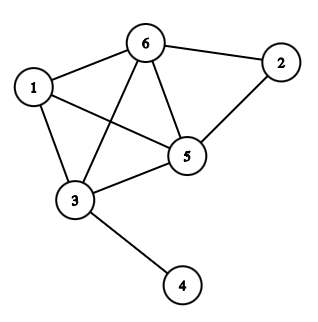
\includegraphics[scale=0.4]{graph.png}
\end{center}

\begin{enumerate}
\item (4 points) Write down the adjacency matrix $A$ for this graph.
\item (4 points) Compute $A^2$ and $A^3$.
\item (5 points)The \textit{Hadamard product} of two $m \times n$ matrices (denoted by $A \circ B$) is entry-wise multiplication (like `\texttt{*}' in NumPy).
  So $(A \circ B)_{ij} = A_{ij} * B_{ij}$ for any indices $i$ and $j$.
  Compute the value of
  \begin{displaymath}
    \frac 1 6 \left(\mathbf 1^T (A^2 \circ A) \mathbf 1\right)
  \end{displaymath}
  (Recall that $\mathbf 1$ is the all-ones vector.
  In the case of this problem, it must be in $\mathbb R^6$.)
\item (5 points) The \textit{trace} of a $n \times n$ matrix (denoted by $\mathsf{tr}(A)$) is the sum of the entries along it's diagonal. So
  \begin{displaymath}
    \mathsf{tr}(A) = A_{11} + A_{22} + \dots + A_{nn}.
  \end{displaymath}
  Compute the value of $\frac 1 6 \mathsf{tr}(A^3)$.
\end{enumerate}
\vfill

\pagebreak
\begin{solution}
\end{solution}

\pagebreak
\section{Regular Stochastic Matrices}
For each of the following stochastic matrices:
\begin{itemize}
\item
  Determine if it is regular.
\item
  Write down a general form solution solution to the homogenous matrix equation $(A - I)\mathbf x = \mathbf 0$).
\item
  If it is possible, find a steady state vector from this solution.
\end{itemize}
For this problem, you may use NumPy as well as code from previous parts of the course.

\begin{enumerate}
\item (6 points)
  \begin{displaymath}
    \begin{bmatrix}
      1 & 1/2 & 1/3 \\
      0 & 1/2 & 1/3 \\
      0 & 0 & 1/3
    \end{bmatrix}
  \end{displaymath}
\item (6 points)
  \begin{displaymath}
    \begin{bmatrix}
      0.9 & 0.9 \\
      0.1 & 0.1
    \end{bmatrix}
  \end{displaymath}
\item (6 points)
  \begin{displaymath}
    \begin{bmatrix}
      0.2 & 0 & 0.3 \\
      0.8 & 0.5 & 0 \\
      0 & 0.5 & 0.7
    \end{bmatrix}
  \end{displaymath}
\end{enumerate}
\medskip

\begin{solution}
\end{solution}

\vfill
\pagebreak
\section{Sonnet Generator (Programming)}

(15 points) In this problem you will be filling in an implementation of a program which uses random walks to generate poetry.
This is based on the idea of the \textit{disocciated press}, a piece of software which does this for arbitrary texts (and which is avaiable in emacs by default).

Large language models like GPT use fancy techniques to predict what word or sequence of words should follow a given piece of text.
It's possible to build a very unfancy version of this using random walks.
Given a corpus of text, we can build a \textit{weighted directed graph} whose nodes are words, and whose edge indicate word adjacency in the corpus.
Each edge can further be labeled with the number of word adjacencies in the corpus.
So words which tend to be next to each other will have larger weights on their edges.

As an example, suppose we used the statement ``a dog and a cat and a bird'' as our corpus.
We can build a graph with nodes for each word (``a'', ``dog'', ``and'', ``cat'' and ``bird'') and with edges for each pair of adjacent words (``a'' to ``dog'', ``dog'' to ``and'', ``and'' to ``a'', and so on).
When we look at the edge from ``and'' to ``a'', it should have weight 2 because ``and a'' appears twice in the statement.

Rather than using a single statement for our corpus, we'll use the entirety of Shakespeare's sonnets.
We will then use this to generate new (nonsense) sonnets by taking a random walk on this graph and collecting words along the way.

The process is roughly as follows:
\begin{itemize}
\item Read in the text of Shakespeare's sonnets and build the adjacency matrix for the graph described above.
\item Convert this matrix into a stochastic matrix by dividing each column by its sum.
  This will make the rest of the implementation easier.
\item Perform a random walk on this matrix, keeping track of the nodes you've visited so far.
\item Use that list of nodes to generate a list of words which will make up the poem.
  Then format that poem so that it can be nicely printed.
\end{itemize}

You are given starter code in the file \texttt{hw06prog.py}.
\textbf{Don't change the name of this file when you submit.}
Also don't change any of the names of functions included in the starter code.
\textbf{The only changes you should make are to fill in the TODO items in the starter code.}
Most of the above process in implemented for you.
All together you have to fill in two functions:
\begin{itemize}
\item \texttt{adjacency\_to\_stochastic} which converts an adjacency matrix into a stochastic matrix by dividing its columns by their sums (\text{Hint.} Make sure to look at and understand \texttt{numpy.sum}).
\item \texttt{random\_walk} which performs a random walk of a given length and returns the list of nodes visited. There is already an implementation of a \textit{single} random step in the function \texttt{random\_step}. You should use this function and collect the outputs into a list.
\end{itemize}
You will upload a single file \texttt{hw06prog.py}.
You will also be provided with a text file \texttt{sonnets.txt} which contains the text of the entirety of Shakespeare's sonnets.
\textbf{You do not need to upload this when you submit}, you just need to upload \texttt{hw06prog.py}.

\end{document}
